\documentclass[main.tex]{subfiles} 
\begin{document}

\section*{Analyse}
\label{sec:2}

Hvordan ble undervisningen lagt opp for å skape god begrepsforståelse i naturfagstimen, og hvordan 
bidro gruppesamtalene til dette? For å svare på dette, la oss se nærmere på hele 
undervisningssekvensen.
\newline
\newline
\subsection*{Aktivisering av forkunnskaper}
Ved oppstarten av timen ble dialog initiert av læreren. Helklassesamtalene hadde preg av
IRE/F metoden (\citeNP{klet13}), dvs. lærer tar initiativ(I), elev responderer(R) og responsen blir 
evaluert(E) og/eller kommentert(F). Til denne sekvensen rekker elevene opp hånda for å respondere. 
Det viser seg at det er noen få elever som er villig til å svare. \citeA[s. 176]{klet13} referer til 
et studie når hun viser til viktigheten av at lærerere legger til rette for \emph{systematisk 
trening, øvelse og bruk av naturfaglige begreper for å utvikle elevenes naturfaglige forståelse, 
inkludert repitisjon av sentrale begreper.}
\newline
\newline
Siden elevene blir spurt om det de har hatt til lekse skal alle elevene skal ha kjennskap til 
begrepene som blir tatt opp og repetert. Det er ønskelig å få bekreftet at elevene innehar en 
overordnet forståelse. Det kan derfor være nødvendig å utpeke noen elever som ikke viser aktiv 
deltagelse i timen og frembringe deres respons. Hvis elevene ikke klarer å respondere på lærer 
initiativ, kan utspørringen av elevene vise hull i deres kunnskap. 
\newline
\newline
Ved å forutse elevsvar før elever i klassen blir initiert, kan misforståelser som 
ofte oppstår bli redegjort av læreren, og respons som ofte opptrer kan tas stilling til. Dette krever 
derimot en god del erfaring fra læreren sin side. I \citeA[s. ~401]{batp08} klassifiseres dette som 
\emph{knowledge of content and students, (KCS)}. Over tid vil en lærer danne omfattende KCS og dette 
kan dermed bidra til å øke kvaliteten på helklassesamtalene. 

\subsection*{Innføring av nytt tema}
Fra figuren \ref{fig:odeg10} kan vi også se at i en vanlig naturfagstime brukes mye tid på å utvikle 
nytt fagstoff.Det kan nok påstås at undervisningsopplegget hadde et preg av mange fagtermer, men 
fokuset i undervisningen var ikke på å innføre fagtermene, men isteden var fokuset å danne forståelse 
om begrepene og deres sammenhenger. 

\begin{figure}[h!]
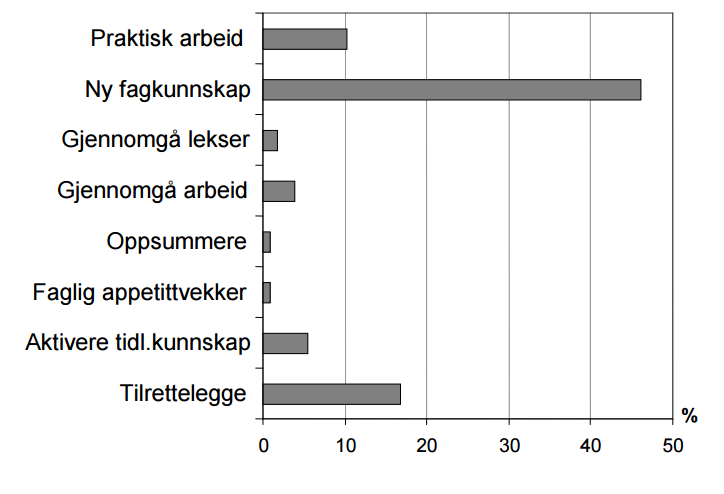
\includegraphics[scale = 0.6]{../figures/undervisnings_aktivitet.png}
\caption{Oversikt over naturfaglærernes undervisningstilbud til elevene fra PISA+ studie. Kilde: \protect\citeA{odeg10}.}
\label{fig:odeg10}
\end{figure}

%gode fagsentrerte samtaler mellom elever hvor elever brukte egne erfaringer
%og språket for å oppnå faglig forståelse, eller faglige samtaler med lærer som hjelper til å skape
%bro mellom praksis og teori 
%\citeA{odeg10}


%  ”inquiry-based science teaching” 
%\citeA{knai11}

\subsection*{Gruppe samtaler}
Siden resterende del av timen skal brukes til repetisjon, er det ikke nødvendig å 
prøve å finne svakheter i elevenes respons gjennom helklassesamtalen. For å finne slike svakheter 
ble gruppesamtalene en bedre plattform. I den forbindelse ble tokolonnenotatet tatt i bruk (se 
vedlegg : \ref{sec:tokolonnenotat}).
\newline
\newline
En viktig del av den sosiale utprøvingen av ideer og begreper innebærer å sammenlikne egne 
forestillinger med andres forestillinger i tillegg til naturvitenskapens forklaringer 
(\citeNP{odeg10}; \citeNP{dals94}). Bruken av tokolonnenotatet i første timen 
\newline
\newline
Evnen til abstrahering henger ifølge Vygotsky (\citeNP[s. 127]{bta98}) med begrepsundervisning, som en
form for vitenskapeliggjøring av hverdagsbegreper. Hvis elever ikke har god begrepsforståelse
kan de ende opp med å bruke naturvitenskapelige begreper i feil kontekst og danne feil 
forbindelser med begrepene. Dette avhenger av deres forkunnskaper. Ausubels kognitive bruer 
(\citeNP[s. 71]{math15}), hans teori om begrepslæring på høyere nivå og hvordan læreren best kan 
legge til rette for slik læring og bruk av begrepene,  handler om å danne forbindelser mellom 
undervisningsmateriell og relevante ideer i elevenes kognitive struktur.
\newline
\newline
Stillasbygging (\citeNP{bta98}; \citeNP[s. 71]{math15})
% Selv om kognitiv forståelse alltid vil være avgjørende viktig i naturfag, så kan vi her spørre om det ikke nettopp er økt evne til deltagelse som bør være 
% begrunnelsen for å utvikle elevenes begrepsforståelse. Fokuset på forståelse må derfor suppleres med vektlegging av lesing for at naturfaget skal forberede til 
% demokratisk deltagelse 
%\citeA[s. ~72]{kols09}

% Slike begreper må være forstått for å kunne ta del i diskusjoner og argumentasjon, og er dermed en del av en naturfaglig allmenndannelse. En slik 
% begrepsforståelse må ses i sammenheng med opplæring i lesing av slike tekster. Ellers kan det være vanskelig å bruke slik kunnskap i nye situasjoner. 
%\citeA[s. ~67]{roen15}


\end{document}